\documentclass[letter,12pt]{article}
\usepackage[letterpaper,right=1in,left=1in,top=1in,bottom=1in]{geometry}
\usepackage{setspace}

\usepackage[utf8]{inputenc}   % allows input of special characters from keyboard (input encoding)
\usepackage[T1]{fontenc}      % what fonts to use when printing characters       (output encoding)
\usepackage{amsmath}          % facilitates writing math formulas and improves the typographical quality of their output
\usepackage[hyphens]{url}     % adds line breaks to long urls
\usepackage[pdftex]{graphicx} % enhanced support for graphics
\usepackage{tikz}             % Easier syntax to draw pgf files (invokes pgf automatically)
\usetikzlibrary{arrows}

\usepackage{mathptmx}           % set font type to Times
\usepackage[scaled=.90]{helvet} % set font type to Times (Helvetica for some special characters)
\usepackage{courier}            % set font type to Times (Courier for other special characters)

\usepackage[longnamesfirst, sort]{natbib}\bibpunct[]{(}{)}{,}{a}{}{;} % handles biblio and references 

\usepackage{rotating}         % sideway tables and figures that take a full page
\usepackage{caption}          % allows multipage figures and tables with same caption (\ContinuedFloat)

\usepackage{dcolumn}          % needed for apsrtable and stargazer tables from R to compile
\usepackage{arydshln}         % dashed lines in tables (hdashline, cdashline{3-4}, 
                              %see http://tex.stackexchange.com/questions/20140/can-a-table-include-a-horizontal-dashed-line)
                              % must be loaded AFTER dcolumn, 
                              %see http://tex.stackexchange.com/questions/12672/which-tabular-packages-do-which-tasks-and-which-packages-conflict


\newcommand{\mc}{\multicolumn}

%% TO ADD NOTES IN TEXT, PUT % BEFORE THE ONE YOU WANT DISABLED
\usepackage[disable]{todonotes}                            % no show
%\usepackage[colorinlistoftodos, textsize=small]{todonotes} % show notes
\newcommand{\emm}[1]{\todo[color=red!15, inline]{\textbf{Eric:} #1}}
\newcommand{\vp}[1]{\todo[color=green!15, inline]{\textbf{Vale:} #1}}
\newcommand{\ges}[1]{\todo[color=blue!15, inline]{\textbf{Ges:} #1}}

\usepackage{xr} % allows cross-ref to other file
\externaldocument{urge15appendix}

%% %for submission: sends figs, tables, and footnotes to last pages
%% \RequirePackage[nomarkers,nolists]{endfloat}     % sends tables and figures to the end
%% \RequirePackage{endnotes}                        % turns fn into endnotes; place \listofendnotes where you want 
%%                                                  %the endnotes to appear (it must be after the last endnote).
%% \let\footnote=\endnote
%% \newcommand{\listofendnotes}{
%%    \begingroup
%%    \parindent 0pt
%%    \parskip 2ex
%%    \def\enotesize{\normalsize}
%%    \theendnotes
%%    \endgroup
%% }
%% 
%% % for submission: drop page numbers when producing title page
%% \pagenumbering{gobble} % Remove page numbers (and reset to 1)
%% \pagenumbering{arabic}% Arabic page numbers (and reset to 1)


% agradecimientos
%% Vidal Mendoza RA
%% Eugenio Solís RA
%% Sonia Kuri RA
%% Ana Lu RU

\setcitestyle{citesep={;}}

\usepackage{listings}

\begin{document}

\title{Speach in Mexico's Cámara de Diputados\thanks{Financial support ITAM, SNI. For shedding light on some parties' internal rules of debate in the period, I am grateful to Fernando Rodríguez Doval, Lupita Vargas Vargas, and one former deputy who wished anonymity. Vidal Mendoza, Eugenio Solís, Sonia Kuri K, ana lu for research assistance.}}
\author{Eric Magar \\ Instituto Tecnológico Autónomo de México}
\date{\today}
\maketitle

\newpage

\begin{abstract}
\noindent Text as data: speaches in lower chamber of Mexico's federal Congress. Analysis covers three pre-midterm election legislative terms since 2006. Argument, findings.\footnote{{Data and supporting materials necessary to reproduce the numerical results in the article are available in the following repository (\url{https://github.com/emagar/legdeb}). Supplementary material for this article is available in the appendix in the online edition.}}
\newline
\newline
\textbf{Keywords}: Speach, Congress, presidentialism, Mexico 
\end{abstract}

\newpage

\doublespacing

\section{Paste in paper}



DV

The statistics above all exclude presiding officers. Presiding officers speak routinely each session but do not engage in debate. One is the chamber president, an officer similar to the Speaker in the UK House of Commons. Diputados are expected to address the chamber president, who is responsible for keeping debate orderly and within chamber and congressional rules. Other officers are secretarios, responsible for formalities such as reading bills, committee reports, or other motions presented to the plenary for consideration, announcing the result of roll call votes, an so forth.  

\singlespacing
\begin{footnotesize}
\begin{verbatim}
| Members in office                                       |   % |    N |
|---------------------------------------------------------+-----+------|
| one observed Legislatura only                           |  86 | 1470 |
| one observed and one or more unobserved Legislaturas    |   9 |  149 |
| two observed (and zero or more unobserved) Legislaturas |   5 |   91 |
| three observed Legislaturas                             |   0 |    0 |
|---------------------------------------------------------+-----+------|
| Total                                                   | 100 | 1710 |
\end{verbatim}
\end{footnotesize}
\doublespacing

The table offers contrast between diputados and presiding officers, adopting members as units instead of daily sessions, as above. Speechless members, who remain unobserved in session-level data, are now accounted for. Of 1,710 members observed across the three Legislaturas, 156 never uttered a single word in the plenary throughout their tenure. The median member spoke 3,677 words in total, the median presiding officer spoke 46,710. Since tenure lengths vary (91 members, or 5 percent of all, were present in two of the Legislaturas observed), a relative measure is desirable. The median diputado spoke 26.4 words per session on average, while the median presiding officer spoke an average 258.6 words per session. Presiding officers are therefore dropped from the analysis. 

95 percent of members never served as presiding officers. Of those who did, the mode was 

\singlespacing
\begin{footnotesize}
\begin{verbatim}
| Years as presiding officer |   % |    N |
|----------------------------+-----+------|
| never                      |  95 | 1630 |
| one                        |   3 |   49 |
| two                        |   1 |   19 |
| three                      |   1 |   12 |
|----------------------------+-----+------|
|                            | 100 | 1710 |
\end{verbatim}
\end{footnotesize}
\doublespacing


\singlespacing
\begin{footnotesize}
\begin{verbatim}
* * Member descriptives for diputados vs presiding officers * *
|                       |  min |   25% |   50% |   75% |    max |
|-----------------------+------+-------+-------+-------+--------|
| DIPUTADOS             |      |       |       |       |        |
| Total words in period |    0 |  1128 |  3677 |  8535 | 242434 |
| Sessions in office    |    1 |   121 |   180 |   201 |    522 |
| Words by session      |    0 |   9.9 |  26.4 |  57.4 | 1212.2 |
|-----------------------+------+-------+-------+-------+--------|
| PRESIDING OFFICERS    |      |       |       |       |        |
| Total words in period | 3141 | 25680 | 46710 | 71669 | 320155 |
| Sessions in office    |   32 |   121 |   182 |   219 |    522 |
| Words by session      | 19.6 | 137.7 | 258.6 | 436.5 | 3563.3 |

* * Member descriptives for diputados vs presiding officers * *
|                       |  min |   10% |   25% |   50% |   75% |    90% |    max |
|-----------------------+------+-------+-------+-------+-------+--------+--------|
| DIPUTADOS             |      |       |       |       |       |        |        |
| Total words in period |    0 |   135 |  1128 |  3677 |  8535 |  16948 | 242434 |
| Sessions in office    |    1 |    25 |   121 |   180 |   201 |    219 |    522 |
| Words by session      |    0 |   1.1 |   9.9 |  26.4 |  57.4 |  109.2 | 1212.2 |
|-----------------------+------+-------+-------+-------+-------+--------+--------|
| PRESIDING OFFICERS    |      |       |       |       |       |        |        |
| Total words in period | 3141 | 13046 | 25680 | 46710 | 71669 | 148511 | 320155 |
| Sessions in office    |   32 |   121 |   121 |   182 |   219 |    227 |    522 |
| Words by session      | 19.6 |  80.9 | 137.7 | 258.6 | 436.5 |  802.0 | 3563.3 |

\end{verbatim}
\end{footnotesize}
\doublespacing


Mexican political system

Mexico has a presidential constitution. For most of the 20th century a hegemonic party, the PRI, controlled the strings of political influence nationwide. While the PRI's electoral fortunes suffered from societal change (ref) and from formidable economic setbacks in the 1980s, it was not until 1997 that competitive politics became the norm. The PRI lost control of the lower house of Congress in that year's midterm election, the first in six decades. Then in 2000 the country's long-standing right-of-center opposition beat the PRI in the presidential race. 

Case selection

Due to time constraints, I afforded cleansing and speech systematization in three legislative terms only: the 60th, 62nd, and 64th Legislatures. Eight have taken place since democratization. I chose pre-midterm election Legislatures, producing temporal discontinuity but likely gaining in case similarity. I also chose the ongoing 64th Legislature (2018-21) instead of the 58th (2000-03) in order to investigate effects of removing single-term member limits in debate. 

This chapter was produced under a hard time constraint, and this determined some methological choices. One was the exclusion of the Senate from analysis. Precedence was given to the Cámara de Diputados because, although the powers of the chambers are symmetric for most legislation, the lower adopts the annual budget without Senate intervention. 

Mexico has a bicameral Congress. The chapter explores the lower chamber only. Although the powers of the chambers are symmetric for most legislation, precedence was given to the Cámara de Diputados because it adopts the annual budget without Senate intervention. 



\subsection{Justify pre-midterm selection}

Exclusion of 61 and 63 was unintentional, time constraints.

But there are good reasons why attention to this sample ok.

Could not go too far anyway (57 58 59 60 61 62 63 64 since democratization). 60 62 64 covers good part.

64 incomplete. Included because first instance of single-party unified government. And, importantly, first Congress where incumbents allowed to be on the ballot in midterm. Plus clear mutation of governing groups after 2+ decades of the partidocracia party system \citep{magar.2007ref.2015,magar.estevez.rosas.2010}. 

Pre-midterm with small N offers control, to the extent that pre- and post-midterm election are different.





\subsection{N speakers}

\begin{figure}
  \centering
    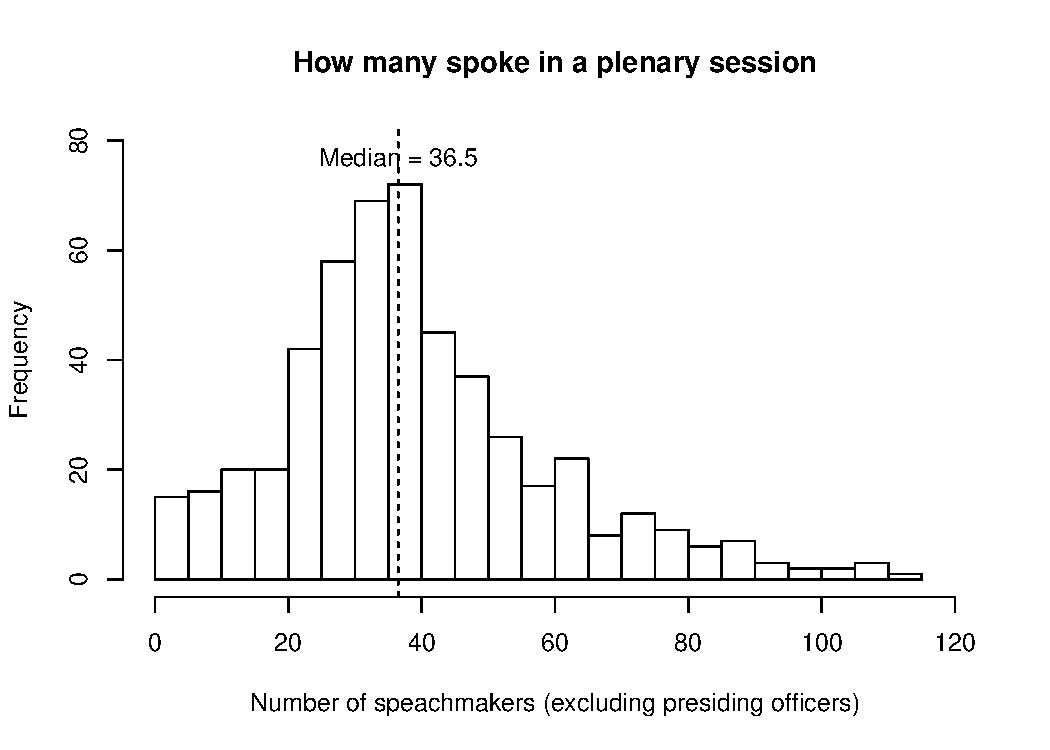
\includegraphics[width=.8\columnwidth]{../plots/nspeakers.pdf}
    \caption{How many spoke in the plenary? Daily plenary sessions of the 60th, the 62nd, and the first two years of the 64th Legislaturas.}\label{F:nspeakers}
\end{figure}





Two DV specifications. 


\section{Multivariate analysis}

The dependent variable is how much a member spoke in plenary debates in a legislative period. Two specifications are analyzed, one absolute, one relative. The absolute *words_(i,p)* is member i's total words in period p. Days where member i spoke less than 50 words in total are considered non-debates, adding zero towards the period's aggregate. The relative specification is *words_(i,p)* divided by the session days that member i served in office as a proportion of all session days in period p. So the denominator for a member who spoke 5 thousand words and served uninterrupted throughtout period p is one, and the two specifications equal 5 thousand. If the member took a leave of absence and served only half of the period the denominator is 0.5, making the relative words equal 5000/0.5=10000.  

The right side of the equation includes explanatory variables in three groups: the member's party, the member's position in the chamber hierarchy, and the member's personal traits. The partisan group includes *majority*, a dummy equal one if the member belonged to the majority party, zero otherwise. Given that one term only had a majority party, the variable indicates Morena party deputies in the 64th Legislature. Expectation. Next is *party size*, the seats that the member's party controlled in the chamber in the term as a proportion of all seats. Since rules allocate speaking time to the parties in proportion to their size, members of smaller parties have more opportunities to speak than  members of larger parties, and the variable should have a negative effect.

A pair of dummies controls for the party's ideology. *Right* equals 1 for members of the right-of-center PAN, 0 otherwise. Left equals 1 for PRD members in 60th and 62nd, and Morena member in the 64th, 0 otherwise. The omitted group includes members of the PRI and the smaller opportunistic parties. The dummy should capture any systematic effect of left's more frequent filibustering attempts. (There is no a priori expectation associated with left and right.)

The chamber hierarchy group includes three explanatory variables. Seniority measures the terms as federal deputy that member i served befre the current term. With single-term limits, members were only eligible to run as diputados for non-consecutive terms, something few did. There are members of two types only in the data, those  

hierarchy

seniority
leader
chair


member

female
(age)
smd
sup


\begin{footnotesize}
  
% Table created by stargazer v.5.2.2 by Marek Hlavac, Harvard University. E-mail: hlavac at fas.harvard.edu
% Date and time: Thu, Jun 11, 2020 - 02:58:25 PM
% Requires LaTeX packages: dcolumn 
\begin{table}[!htbp] \centering 
  \caption{Regression results} 
  \label{} 
\begin{tabular}{@{\extracolsep{5pt}}lD{.}{.}{-2} D{.}{.}{-2} D{.}{.}{-2} D{.}{.}{-2} D{.}{.}{-2} } 
\\[-1.8ex]\hline 
\hline \\[-1.8ex] 
 & \multicolumn{5}{c}{\textit{Dependent variable:}} \\ 
\cline{2-6} 
\\[-1.8ex] & \multicolumn{2}{c}{Words in period} & \multicolumn{3}{c}{Words in period (relative to tenure)} \\ 
\\[-1.8ex] & \multicolumn{2}{c}{\textit{negative}} & \multicolumn{2}{c}{\textit{OLS}} & \multicolumn{1}{c}{\textit{linear}} \\ 
 & \multicolumn{2}{c}{\textit{binomial}} & \multicolumn{2}{c}{\textit{}} & \multicolumn{1}{c}{\textit{mixed-effects}} \\ 
\\[-1.8ex] & \multicolumn{1}{c}{(1)} & \multicolumn{1}{c}{(2)} & \multicolumn{1}{c}{(3)} & \multicolumn{1}{c}{(4)} & \multicolumn{1}{c}{(5)}\\ 
\hline \\[-1.8ex] 
 Tenure (logged) & 0.94^{***} & 0.97^{***} &  &  &  \\ 
  & (0.04) & (0.04) &  &  &  \\ 
  & & & & & \\ 
 Majority & 0.73^{***} & 0.67^{***} & 4,476.27^{***} & 5,258.27^{***} & 4,145.80^{***} \\ 
  & (0.11) & (0.17) & (292.98) & (351.82) & (562.84) \\ 
  & & & & & \\ 
 Party size & -5.10^{***} & -5.04^{***} &  &  &  \\ 
  & (0.21) & (0.24) &  &  &  \\ 
  & & & & & \\ 
 Right &  &  & -1,162.20^{***} & -1,546.63^{***} & -1,359.04^{***} \\ 
  &  &  & (59.95) & (71.42) & (117.24) \\ 
  & & & & & \\ 
 Left & 0.01 & 0.09 & -65.14 & 94.10 & 81.06 \\ 
  & (0.07) & (0.07) & (77.06) & (77.01) & (143.66) \\ 
  & & & & & \\ 
 Seniority & 0.28^{***} & 0.33^{***} & 12.87 & 135.88^{*} & 156.55 \\ 
  & (0.08) & (0.08) & (77.05) & (78.17) & (137.38) \\ 
  & & & & & \\ 
 Party leader & 0.17^{***} & 0.18^{***} &  &  &  \\ 
  & (0.05) & (0.05) &  &  &  \\ 
  & & & & & \\ 
 Comm. chair &  &  & 363.47^{***} & 287.16^{***} & 435.96^{***} \\ 
  &  &  & (83.26) & (82.49) & (117.33) \\ 
  & & & & & \\ 
 SMD & 0.42^{**} & 0.40^{*} & 2,316.93^{***} & 2,386.04^{***} & 1,469.52^{***} \\ 
  & (0.21) & (0.21) & (210.89) & (208.99) & (319.39) \\ 
  & & & & & \\ 
 Suplente & 0.35^{***} & 0.32^{***} & -86.78 & 104.10 & 64.28 \\ 
  & (0.09) & (0.09) & (92.38) & (92.10) & (155.50) \\ 
  & & & & & \\ 
 62nd Leg. & -0.04 & -0.04 & -294.59^{***} & -186.99^{***} & -235.74^{**} \\ 
  & (0.06) & (0.06) & (56.81) & (56.81) & (98.74) \\ 
  & & & & & \\ 
 64th Leg. & -0.34^{***} & -0.33^{***} & -464.64^{***} & -388.86^{***} & -287.62^{**} \\ 
  & (0.11) & (0.11) & (113.82) & (112.58) & (144.75) \\ 
  & & & & & \\ 
 Female &  & 0.23^{***} &  & -691.36^{***} & -484.89^{***} \\ 
  &  & (0.06) &  & (76.88) & (122.93) \\ 
  & & & & & \\ 
 Constant &  & 0.18^{*} &  & 635.84^{***} & 911.97^{***} \\ 
  &  & (0.10) &  & (94.29) & (145.71) \\ 
  & & & & & \\ 
 dfem & 0.08 & 0.06 & 98.66^{*} & 114.92^{**} & 9.78 \\ 
  & (0.06) & (0.06) & (56.66) & (56.59) & (102.72) \\ 
  & & & & & \\ 
 Constant & 2.57^{***} & 2.31^{***} & 2,720.24^{***} & 3,180.82^{***} & 2,946.45^{***} \\ 
  & (0.15) & (0.17) & (75.42) & (105.36) & (166.74) \\ 
  & & & & & \\ 
\hline \\[-1.8ex] 
Observations & \multicolumn{1}{c}{9,494} & \multicolumn{1}{c}{9,494} & \multicolumn{1}{c}{9,494} & \multicolumn{1}{c}{9,494} & \multicolumn{1}{c}{9,494} \\ 
R$^{2}$ &  &  & \multicolumn{1}{c}{0.10} & \multicolumn{1}{c}{0.12} &  \\ 
Adjusted R$^{2}$ &  &  & \multicolumn{1}{c}{0.10} & \multicolumn{1}{c}{0.12} &  \\ 
Log Likelihood & \multicolumn{1}{c}{-60,817.31} & \multicolumn{1}{c}{-60,811.57} &  &  & \multicolumn{1}{c}{-85,479.08} \\ 
$\theta$ & \multicolumn{1}{c}{0.16^{***}  (0.002)} & \multicolumn{1}{c}{0.16^{***}  (0.002)} &  &  &  \\ 
Akaike Inf. Crit. & \multicolumn{1}{c}{121,658.60} & \multicolumn{1}{c}{121,651.10} &  &  & \multicolumn{1}{c}{170,988.20} \\ 
Bayesian Inf. Crit. &  &  &  &  & \multicolumn{1}{c}{171,095.50} \\ 
Residual Std. Error &  &  & \multicolumn{1}{c}{2,578.64 (df = 9483)} & \multicolumn{1}{c}{2,547.33 (df = 9481)} &  \\ 
F Statistic &  &  & \multicolumn{1}{c}{105.02$^{***}$ (df = 10; 9483)} & \multicolumn{1}{c}{109.40$^{***}$ (df = 12; 9481)} &  \\ 
\hline 
\hline \\[-1.8ex] 
\textit{Note:}  & \multicolumn{5}{r}{$^{*}$p$<$0.1; $^{**}$p$<$0.05; $^{***}$p$<$0.01} \\ 
\end{tabular} 
\end{table} 

\end{footnotesize}

\begin{figure}
  \centering
    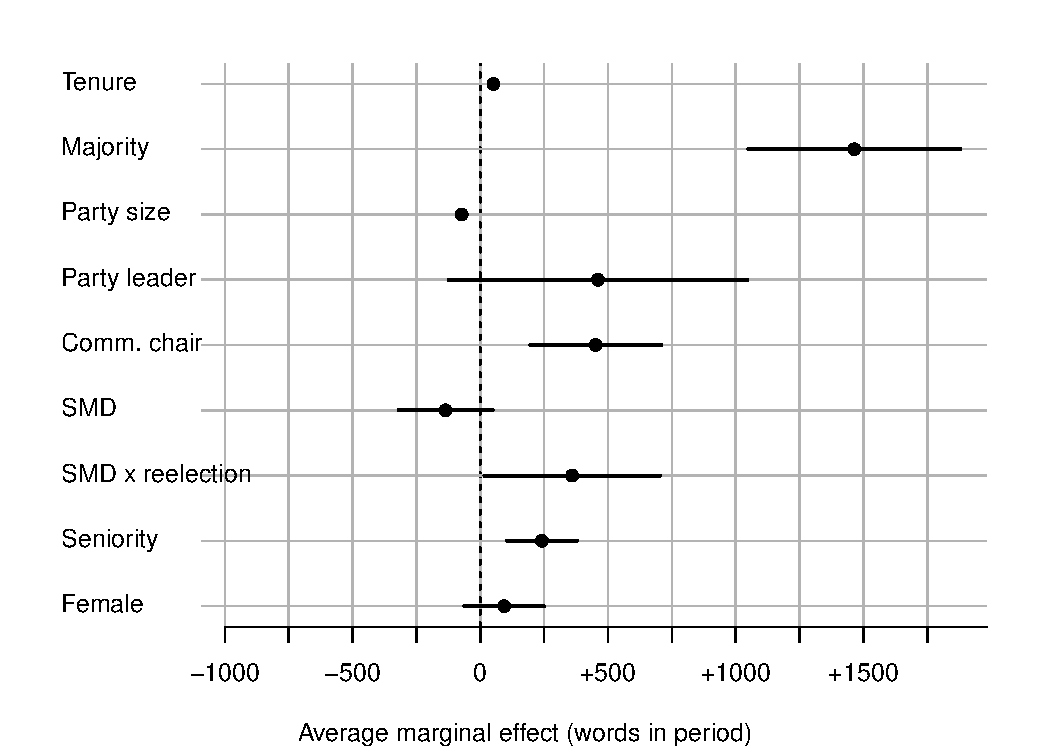
\includegraphics[width=.8\columnwidth]{../plots/avgMgEffects.pdf}
    \caption{Average marginal effects from model 5. Dots report the effect in expected period speech length of a unit change in each independent variable, all else at mean values; bars are 95-percent confidence intervals.}\label{F:avgmgeff}
\end{figure}

%% model 5 (fit2 in code) average marginal effects
%%      factor       AME       SE        z      p     lower     upper
%%  ev.pot.dys   51.3100   2.6546  19.3285 0.0000   46.1070   56.5129
%%        dmaj 1464.4438 211.4850   6.9246 0.0000 1049.9408 1878.9469
%%    size.maj  -72.7583   4.9124 -14.8113 0.0000  -82.3863  -63.1303
%%     dleader  460.6492 298.1915   1.5448 0.1224 -123.7954 1045.0937
%%      dchair  451.9050 130.7671   3.4558 0.0005  195.6061  708.2039
%%        dsmd -135.7903  93.9759  -1.4449 0.1485 -319.9796   48.3991
%%      dsmd64  359.7821 175.2500   2.0530 0.0401   16.2985  703.2657
%%   seniority  241.5023  69.7417   3.4628 0.0005  104.8111  378.1935
%%        dfem   93.4748  79.3548   1.1779 0.2388  -62.0578  249.0074
%%        dsup -507.2173 160.3330  -3.1635 0.0016 -821.4642 -192.9703
%%         d62  259.0260  89.6724   2.8886 0.0039   83.2712  434.7807
%%         d64 -132.3693 165.2884  -0.8008 0.4232 -456.3285  191.5899

Figure \ref{F:avgmgeff} reports changes in the average predicted number of words associated with unit changes in explanatory variables. This exercise uses model 5 estimates. By translating into interpretable quantities, marginal effects are a convenient way to gauge negative binomial regression coefficients. It is clear in the plot that the larges effect is attributable to majority status. Other things constant (at mean values), members in the majority party each spoke between about 1,000 and 1,900 more words per period than the rest of the chamber. Multiplication of that average by Morena's 254 members in the 64th Legislatura produces 372 thousand additional words---47 percent of all words in the median ordinary period.

The report from a committee with a coalition chair experiences a 0.17
hike (0.06 standard error) in the likelihood of receiving a closed rule compared to a report by an
opposition-chaired committee. The effect is as big as the average marginal effects of Hacienda
Referral (0.18), which capures mostly high-significance draft laws, and that of Multiple Referrals
(0.16), which we view as an indicator of issue complexity. We therefore find no statistical evidence
to reject our Hypothesis 1. The results also confirm hypothesis 2, showing that a bill reported by a
generally less friendly committe (chaired by the opposition), has a higher probability of receiving
an open rule on the floor, thereby allowing the floor majority to bring back the bill to the median
through floor amendments. Thus, presidents use open rules to control bills coming from preference
distant committee chairs.
The substantial effects of Hacienda Referral and Multiple Referrals deserve comment. They
suggest, first, that when spending gets in the way, restrictive rules are the norm in Chile. Recall
that Multiple Referrals exclude the Finance Committee, so there is an independent effect of bills
with jurisdictional overlaps worth investigating further, and which must be associated, in part at
least, to influencing the report through a friendlier committee. 16 Furthermore, note that the Finance
Committee was always chaired by a coalition member but, with the exception of the 1998–2000
period, never by a co-partisan of the president. This may explain the milder effect of the partisan
specification of our key variable in model 1.
Another effect worth highlighting is Introd. in Senate. Bills successfully passing the Upper
Chamber first, where the opposition was systematically larger and attimes in control, were much
less likely to get urgent status (the average marginal effect is −0.15 and significant). This suggests
that agreements and compromises reached in the Senate ignited less, not more, protection from
floor amendments in the Cámara’s plenary, most likely as a consequence of the greater prefer-
ence divergence between the President and the opposition-led Senate. Analysis of inter-chamber
negotiation and the reliance on urgency in the Upper Chamber are interesting venues for future
research.
Finally, there are time trends in fast-track authority that simulations reveal neatly. Figure 5
portrays the predicted probability that a bill enters the fast-track throughout the legislative year.
Regressors in model 3 are held constant to simulate a bill sent to the Cámara in the 2006–10
Legislature that was referred to a single committee, excluding Hacienda. Presidential Approval
(insignificant across models) is set to the mean for President Bachelet’s first term, coinciding in full
with the 2006–10 Legislature. The inverted-U shape shows how fast-track probability, predicted
at 0.17 for coalition-chaired committees at the start, and 0.08 for the rest, becomes much likelier
in the first half of the legislative year. By the second quarter (June–August), the probability is at
its peak, about 0.32 percent and 0.17, respectively. It then experiences a sharp drop, ending the
austral Summer break at 0.13 for coalition-chaired committees, and 0.05 for others. And while 95-
percent confidence bands overlap, they barely do so at the middle of the legislative year, lending
confidence that we are picking up a signal and not just random noise.


\section{Predicted words}

\begin{figure}
  \centering
    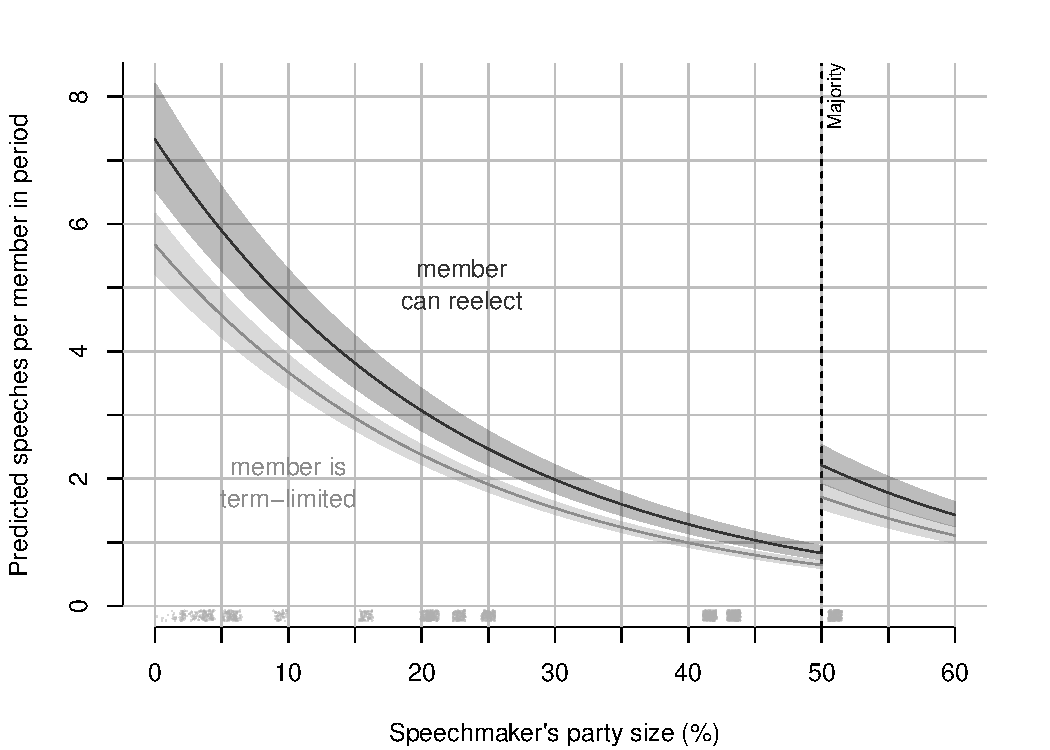
\includegraphics[width=.8\columnwidth]{../plots/predictedWords.pdf}
    \caption{Predicted speech length. Lines report point predictions using model 5.}\label{F:predict}
\end{figure}




\section*{Acknowledgements}
Eric Magar received financial support from the Asociaci\'on Mexicana de Cultura \textsc{a.c.}\ and \textsc{conacyt}'s Sistema Nacional de Investigadores. The author is grateful to Ana Lucía Enríquez, Eugenio Solís Flores, Vidal, Sonia for research assistance.  The author are responsible for mistakes and shortcomings in the study.

\listofendnotes

\bibliographystyle{apsr}

\bibliography{../bib/magar}

%% \begin{thebibliography}{xx}

%% \harvarditem{Alem\'an \harvardand\ Tsebelis}{2016}{aleman-tsebelis-2016-book}
%% Alem\'an, Eduardo \harvardand\ George Tsebelis. 2016.
%% \newblock {\em Legislative Institutions and Lawmaking in Latin America}.
%% \newblock Oxford:  Oxford University Press.

%% \harvarditem{Alem\'an \harvardand\ Navia}{2009}{aleman.navia.UrgChi.2009}
%% Alem\'an, Eduardo \harvardand\ Patricio Navia. 2009.
%% \newblock ``Institutions and the Legislative Success of `Strong' Presidents: An
%%   Analysis of Government Bills in {Chile}.'' {\em Journal of Legislative
%%   Studies} 15(4):401--19.

%% \end{thebibliography}


\end{document}

